\documentclass{article}
\usepackage{graphics}
\usepackage{graphicx}
\usepackage{tabularx}
\usepackage[titletoc,title]{appendix}

\title{GEp SBS trigger update}

\author{A. Camsonne, M. K. Jones}

\begin{document}
\maketitle
\section{Experiment overview}
The proton form factor, GEp, experiment measures elastic electron-proton scattering. For electron
detection, a large lead glass calorimeter, ECAL,  will be used with the Coordinate Detector, CDET, placed in front
of ECAL.  The CDET is primarily used
to make a high precision measurement of the electron out-of-plane angle. The proton will be
detected in the SBS spectrometer which consist of front tracker INFN GEMs, a polarimeter and the hadron calorimeter, HCAL.
The front tracker will consist of 6 INFN GEM chambers ( each GEM INFN chamber is 3 GEM modules of 40x50cm$^2$).
The polarimeter consists of two groups of 5 University of Virginia GEM chambers (each UVa GEM chamber
is 4 GEM modules of 60x50cm$^2$). The trigger will be a coincidence between the ECAL and HCAL.

The front 4 GEM chambers are being built by INFN group. Each chamber consists
of 3 GEM modules. Each GEM module covers an area of 40x50 cm$^2$. The readout plane is pitched at 400~$\mu$m
and is readout using 128 channel APV25 chips. Each module is readout by a total of 18 APV25 chips ( 8 along
the 40~cm and 10 along the 50~cm). So a GEM front chamber has 6912 channels which gives a total of 27648 channels
for the 4 GEM chambers. The APV25 chips will be readout by a VME64x/VXS Multi-Purpose Digitizer (MPD) that was
develop by an INFN group.

The rear GEM chamber is being built by the University of Virginia and is part of the toal of 10 GEM chambers
that will be used as the rear tracker for the GEp experiment. Each chamber consist of 4 GEM modules.
Each GEM module covers an area of 60x50 cm$^2$ and are combined into a chamber with an area
of 60x200 cm$^2$. The readout plane is pitched at 400~$\mu$m.
 Readout is done using 128 channel APV25 chips. Each module is readout 
by a total of  22 APV25 chips (  12 along the 60~cm and 10 along the 50~cm). So a GEM rear chamber has  
11264 channels which gives a total of 112,640 channels for the 10 GEM chambers. The readout of the GEM
rear chamber APV25 chips will use the same INFN MPD electonics as the front GEM chambers. 

ECAL is a large array of 1710 lead glass bars that are available from the
previous proton form factor experiment, GEp3, that was run at JLab in 2008.
The electronics and cabling from past JLab experiments will be re-used. The 
lead glass bars will be readout out by  FASTBUS 1881M 64 channel ADC modules. As done in the GEp3 experiment,
the analog signals from 8 blocks will be summed together in groups of 2x4 using custom built ``summing'' modules.
The ``summing'' modules have two sets of eight inputs. Each set of eight inputs is summed together
and six summed analog outputs for each group of eight are available. In addition the ``summing'' module 
produces the 16 individual
analogs signal with an amplification of 4.2 that can be sent to an ADC. There will be 1710 individual blocks.
Other analog outputs from the  ``group of 8'' would be sent to additional
FI/FO units to form summed analog signal from a group of 32 blocks to be used in the ECAL trigger as
explained in Section~\ref{sec:ecal-trig}.





The hadron calorimeter, HCAL, is a 12x24 block array which will be readout 
by a JLab FADC250, a 16-channel 12-bit Flash 
ADC sampling at 250 MHz.  The FADC250 is readout through the VXS pipelined electronics. HCAL will be the proton singles trigger as explained in Section~\ref{sec:hcal-vxs}.


The Coordinate Detector is  two planes of scintillator. Each plane consist of 1176 scintillator bars. 
Each scintillator bar is readout by a wavelength shifting fiber. Fourteen of the WLS  will be coupled to
a 16 channel multianode PMT. Each analog output of the PMT will be input to a 16 channel amplifier/discriminator
card base on the NINO chip. The logic signals from the NINO chip will go to FASTBUS 1877s 96 channel TDC modules.
Since the CDET is using only 14/16 channels , space is need for 2688 TDC channels ( 16/14*2352).

\section {Trigger}

\subsection{ECAL trigger}
\label{sec:ecal-trig}
In Fig.~\ref{fig:ECALTrig}, the left plot shows the distribution of events at the front of the ECal
and overlayed on the individual blocks. The middle plot shows the groups of 2x4 blocks ( outlined in red)
which will go into the sum of 8 modules. Around the edges the groups include less than 8 blocks 
(outlined in green). There are a total of 219 sum of 8 modules needed.
The sum of 8 modules pass the individual analog signal of each block to a connector in the
back of the module. A cable goes from this connector goes to a nearby patch panel on the ECal platform. The patch panel goes to a long 500ns delay cable which brings the signal to
another patch panel in the electronics hut. This patch panel changes from the individual BNC cables into a 16 channel ribbon cable which goes into the 1881M ADC. 
Table~\ref{tab:ECALadctime} gives the total propagation time of the individual signal from each block along with the breakdown into the different components.
\begin{figure}
	\centering
	% Requires \usepackage{graphicx}
	\includegraphics[width=0.3\textwidth]{cfpbox.pdf}
	\includegraphics[width=0.3\textwidth]{cfpc.pdf}
	\includegraphics[width=0.3\textwidth]{cgr32.pdf}
	\caption{The left plot is the distribution of elastic electrons in ECAL with the black rectangles representing the 1710 blocks. The middle plot demonstrates
		the scheme for make groups of 2x4 lead glass blocks to be used in the ECAL trigger. The right plot is the same as the middle plot but without the individual blocks to make it easier to see.}\label{fig:ECALTrig}
\end{figure}
\begin{table}[b]
	\begin{tabular}{|l|l|} \hline
		Cable length from PMT to sum of 8 module & 40ns \\ \hline
		Sum of 8 module transit time & 10ns \\ \hline
		Cable from back of the Sum of 8 module to patch panel on ECal & 6ns \\ \hline
		Cable from ECal patch panel to patch panel in electronics hut & 500ns \\ \hline
		Ribbon Cable from patch panel on ECal & 15ns \\ \hline
		Total time & 571ns \\ \hline  		   		  		 		 
	\end{tabular}
	\caption{The contributions to total propagation time  of the ECal calorimeter signals.}
	\label{tab:ECALadctime}
\end{table}



For the formation of the trigger, the sum of 8 modules have 6 outputs of the summed signal.
In the right plot of Fig.~\ref{fig:ECALTrig}, the groups of 32 blocks which sum 4 groups of
8 blocks are indicated by purple filled circles at the intersection of 4 groups of 8. 
The group of 32 blocks overlap
by two groups of 8 in both horizontal and vertical directions. So most of the
groups of 8 have to go to 4 groups of 32. At the edges the groups of 8 feed into
two groups of 32. There are 192  groups of 32. The output of the groups of 32 would go into 16 channel
discriminators. A total of twelve 16-channel discriminators will be used.
The discriminators are existing Phillips 707 units which have both 
16 LEMO and 16 ECL output. The  LEMO outputs of the
discriminator would go into a 16-channel mixed logic unit to produce an "OR" for each set of
16 inputs. The 12 "OR" signals would go into a final 16-channel mixed logic unit to 
a trigger that needs to be sent to the Trigger Supervisor as the Level One trigger. A 50m fast R8 cable will bring the trigger from the ECal platform to the Trigger Supervisor
which will be located in a VXS crate in the electronics hut. The Trigger Supervisor
takes 40ns to produce the ADC gate and the cable from the Trigger Supervisor to the
trigger distribution card in the back of the FASTBUS crate takes 25ns. The total time
is 391ns which is 180ns less than the 571ns for the propagation time of the individual
signals to the ADC.

To form the coincidence trigger, the ECL output of the discriminators for the 192 
ECal groups of 32 have to be sent to a VME crate via  twelve ribbon cables.
The signals will be sent to a VXS pipelined input register, called VETROC, which
can have up to 208 logic inputs which a 1 ns timing resolution. 
These signals can then be sent to a VXS Global Trigger Processor unit which
forms the coincidence trigger as explained in Section~\ref{sec:hcal-vxs}.


\begin{table}
	\begin{tabular}{|l|l|} \hline
		Cable length from PMT to sum of 8 module & 40ns \\ \hline
		Sum of 8 module transit time & 10ns \\ \hline
		Cable from Sum of 8 module to FI/FO for group of 32 & 24ns \\ \hline
		FI/FO module transit time & 10ns \\ \hline
		Cable from FI/FO to the 16 channel discriminator & 4ns \\ \hline
		16 channel discriminator  transit time & 10ns \\ \hline
		Cable from the 16 channel discriminator to 16 channel mixed logic unit& 4ns \\ \hline
		16 channel mixed logic unit  transit time & 10ns \\ \hline
		Cable from the 16 channel mixed logic units to final 16 channel mixed logic unit& 4ns \\ \hline
		16 channel mixed logic unit  transit time & 10ns \\ \hline
		50M fast cable from the ECal platform to Trigger Supervisor & 200ns \\ \hline
		Transit time in TS to produce the ADC gate & 40ns \\ \hline
		Cable from TS to logic fan  & 6ns \\ \hline\hline
		Logic fan  & 10ns \\ \hline\hline
		Logic fan to FASTBUS crate & 25ns \\ \hline\hline
		Total time & 407 ns \\ \hline  		   		  		 		 
	\end{tabular}
	\caption{The contributions to total time formation of the ECal Level One trigger sued as the ADC gate.}
	\label{tab:ECALTrigtime}
\end{table}


\begin{figure}
		\centering
	 
\includegraphics[scale=0.8,angle=90]{figs/GeP.pdf}
 	\caption{ECal Trigger Timing Diagram.  }
 	\label{fig:ECALTrigDiag}
 	\end{figure}
 	
 	\newpage
\section{HCAL trigger}
\label{sec:hcal-vxs}
The hadron calorimeter will be read out by the JLAB pipelined electronics.
The central module for this system is the JLAB FADC250, a 16-channel 12-bit FADC sampling at 250~MHz. The input signals are continuously recorded into the memory with a memory depth up to 8 us. The system is thus dead timeless as long as the trigger is generated before the memory rolls over and the event of interest is overwritten.
The Flash ADC has two separated data path.
The first one uses the new high speed serialized VME standard called VME switched Serial (VXS).
It allows full duplex point to point connection at up to 2.5 Gbps per lane using the backplane central connector.
Currently the FADC is using two VXS lanes giving 5 Gbps of bandwidth.
This allows to transfer a 16 bit word from each FADC to a Crate Trigger Processor (CTP) board every 4~ns.
Each FADC being connected to The CTP via a 5 Gbps link, the CTP uses up to 16 FADC words from each FADC to form a 32-bit word every 4~ns which can be a lower resolution sum of all the channels or a bit pattern of the channel hit for example.
The CTP board then sends the processed signals to a Sub-System Processor (SSP) board via a 10 Gbps optical link which puts together all the data from individual crates and computes the associated quantities which will be used in the trigger.
All the SSP boards send their processed information to a Global Trigger Processor (GTP) which makes the L1 trigger.
The GTP sends the trigger to the Trigger Supervisor (TS) which makes sure the system is ready to accept a trigger and sends the accepted signal to the Trigger Distribution boards in the VXS crates which are linked to the Trigger Interface boards in each crates via optical link as represented in Fig.\ref{fig:pipeline_daq}.
The trigger and synchronization clock signals will then be sent back to individual crates and payload modules through Trigger Interface/Distribution (TID) boards and Signal Distribution (SD) boards which distributes the signals to the electronics such as the FADC.
Once a trigger is generated, the full resolution data which is still in the pipeline is readout out using the VME320 protocol at an average data rate of 200 MB/s.
The Flash ADC can run in different modes, it can either transfer all the samples of the waveform which can be useful to study pileup effect and background or process the data to give an integral over the length of the pulse. In both mode, a threshold can be put on each individual channel to reduce the data.

\begin{figure}
	\centering
	% Requires \usepackage{graphicx}
	\includegraphics[width=\textwidth]{figs/TriggerPipeline.pdf}\\
	\caption{Standard Triggering scheme using the JLAB pipeline electronics}\label{fig:pipeline_daq}
\end{figure}

The GTP having all the amplitude of all the calorimeter, it can compute all the sums of adjacent blocks.
A sum of 3$\times$3 blocks was implemented for the heavy photon search experiment (HPS).
In order to reduce the number of triggers coming from the background this summing approach is chosen to improve the online pion rejection.
A sum over 4x4 adjacent blocks can be implemented in the same way as the HPS scheme. 

\begin{figure}
	\centering
	% Requires \usepackage{graphicx}
	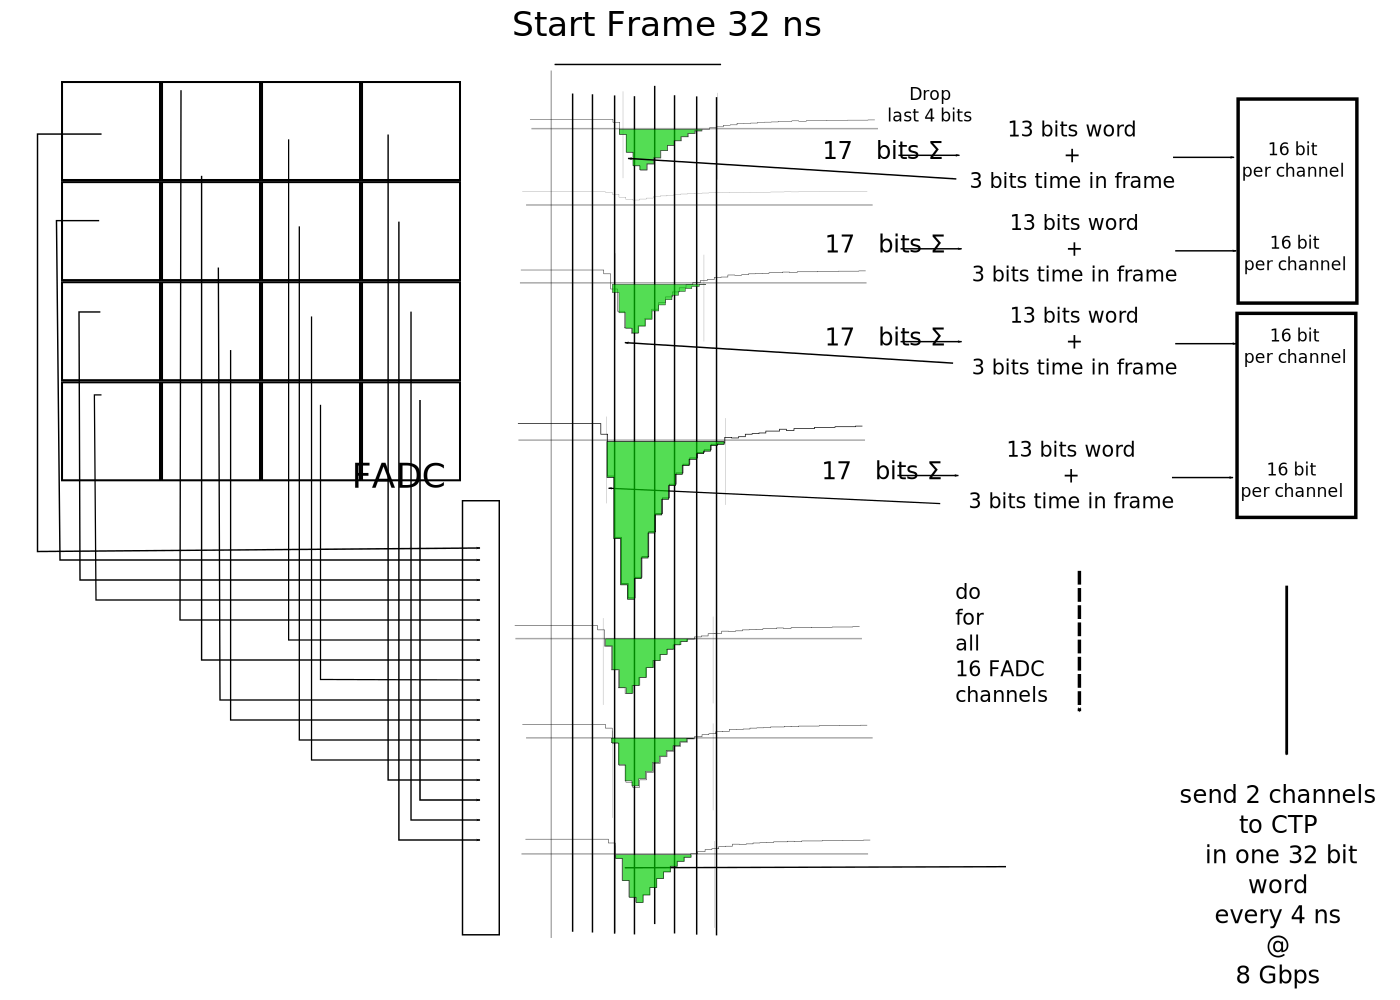
\includegraphics[width=\textwidth]{figs/CaloTrigger.pdf}
	\caption{Calorimeter clustering scheme using the HPS algorithm. All calorimeter signals are sent to the FADC. }\label{fig:ClustHPS}
\end{figure}

\begin{figure}
	\centering
	% Requires \usepackage{graphicx}
	\includegraphics[width=\textwidth]{figs/HCALSum.pdf}
	\caption{All sum of 4x4 are computed, if one is above threshold L2 is generated }
\end{figure}

\begin{figure}
	\centering
	% Requires \usepackage{graphicx}
	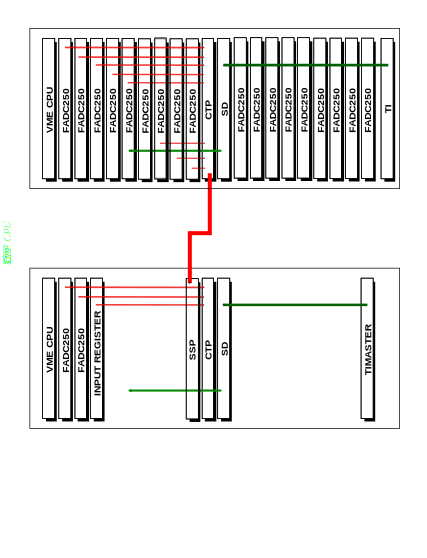
\includegraphics[width=\textwidth]{figs/VXSHCalFADC.pdf}\\
	\caption{HCAL crate layout }\label{fig:HCALFADC}
\end{figure}

Since we have 288 channels for the HCAL, 18 FADCs will be used using two VXS crates. The crate with all 16 FADCs will send its data ti theother CTP through the SSP using the 10 Gb/s optical link. The second crate will hold the two additionnal FADCs and a pipelined input register called VETROC which can have up to 208 logic inputs which a 1 ns timing resolution, to send the sums firing in the ECAL to the GTP to generate the L2 using the geometrical matching of the HCAL with the ECAL. The total process will not take more than 1 $\mu s$ which is sufficiently fast for the APVs which have a look back of 4 $\mu s$.

\section{Electronics inventory}
\label{sec:inventory}
\subsection{Pipelined electronics}
\label{sec:pipe}
\subsubsection{JLab Flash ADC 250}
The JLab Flash ADC 250 is a VME 12 bit 250 MHZ Flash ADC with 16 channels. It can transfer data through the VME64X backplane in 2eSST protocol which can reach up to 200 MB/s, it can also transfer data through the VXS backplane which is serial multiline point to point protocol with data transfer up to 8 GBit/s per lane. Each FADC has 4 VXS lanes. It has 8 microsecond pipeline. It will be used for the Hadron Calorimeter readout to allow to produce a HCAL trigger by doing clustering of the FADC data in a dedicated logic module the VXS Trigger Processor (VTP).  
\subsubsection{F1 TDC}
The JLAB F1 TDC is base on the F1 chip, it is a pipelined multihit pipelined TDC with 64 channels in low resolution mode 120 ps and 32 channel in high resolution mode of 60ps. It can be readout using the VME backplane also using the 2eSST transfer protocol for data rates up to 200 MB/s. It will be used for Neutron Form Factor experiment where the neutron momentum is measured by time of flight. The F1 TDC will supplement the FADC which typically can give a timing resolution of 0.3 ns.
\subsubsection{SubSystem Processor}
The SubSystem Processor is part of the standard JLAB pipeline electronics system. It is a VME64X board with 8 QSFP optical port with VME 2eSST capability (200 MB/s) and VXS connectivity.
The initial goal of the SSP was to gather data from different crates of FADC to concentrate the data to a single logic module Global Trigger Processor (GTP) which is superseded by the VXS Trigger Processor (VTP). Each optical link can transfer up 6.25 Gb/s giving a 25 GBit/s bandwidth for each QSFP connector the board can send data to the VTP using up to 4 VXS lines with each line having a 6.25 Gbit/s bandwith.
Since this module is capable of reading a lot of data in parallel it will also be used to readout the GEM electronics using their optical cable. Data processing for improved zero suppression will be done by the SSP FPGA.
\subsubsection{VETROC}
The VXS Electron Trigger Read Out Controller (VETROC) is a board to generate an electron trigger from a silicton strip detector. It was designed as a flexible 192 channels pipelined input output/register compatible with JLAB pipeline electornics system. It allows to have the status of each of its input at 250 MHz sampling which can be used for trigger purpose in conjunction with the FADC data.

\subsubsection{VXS Trigger Processor}
The JLAB pipeline system relies on the VXS bus to transfer the FADC data to a central module called General Trigger Processor (GTP) where the logic involving all the FADC channels can be processed. A new version of this module with additionnal optical link on the front panel and VXS lines on the back was designed and called VXS Trigger Processor (VTP).


\subsection{Fastbus electronics}
\subsubsection{Lecroy 1881M ADC}
The electromagnetic calorimeter having a large number of channel will be readout using the Fastbus 1881M.
It is a high Density, 64 Channels Per FASTBUS Slot 13 bit integrating ADC. It has a conversion Time of 12 µsec in 13-Bit Mode (9 µsec in 12-Bit Mode) a fast clear is possible to allow a L1 L2 logic reducing the dead time due to conversion. It can be programmed to perform online pedestal suppression. It has a buffer up 64 Events.
Theoretical data transfer is up to 40 MB/s with an actual sustained rate of 15 MB/s.
A fast clear can be issued and the module is ready to register another trigger after 1 $\mu$s.

\subsubsection{Lecroy 1877S TDC}
All other hit based detectors (CDET, GRINCH) will be read with Fastubs 1877S Multihit Time-to-Digital Converter with Data Supression.It is a  High Density, 96 Channels Per FASTBUS Slotwith 0.5 ns resolution.
It is a multhit TDC with up to 16 Hits/Channel and it can detect rising and/or falling edge which will allow to measure the amplitude of the signal with time over threshold information. It can hold up to 8 events in its buffer. The module can define windows for signal to be recorded in 4ns steps reducing the amount of data from accidentals. It can hold up to 8 Events in its buffer.
    Fast clear after 1 $\mu$s 300 ns after stop.

\begin{appendices}
	

%\subsection{Hall layout}
%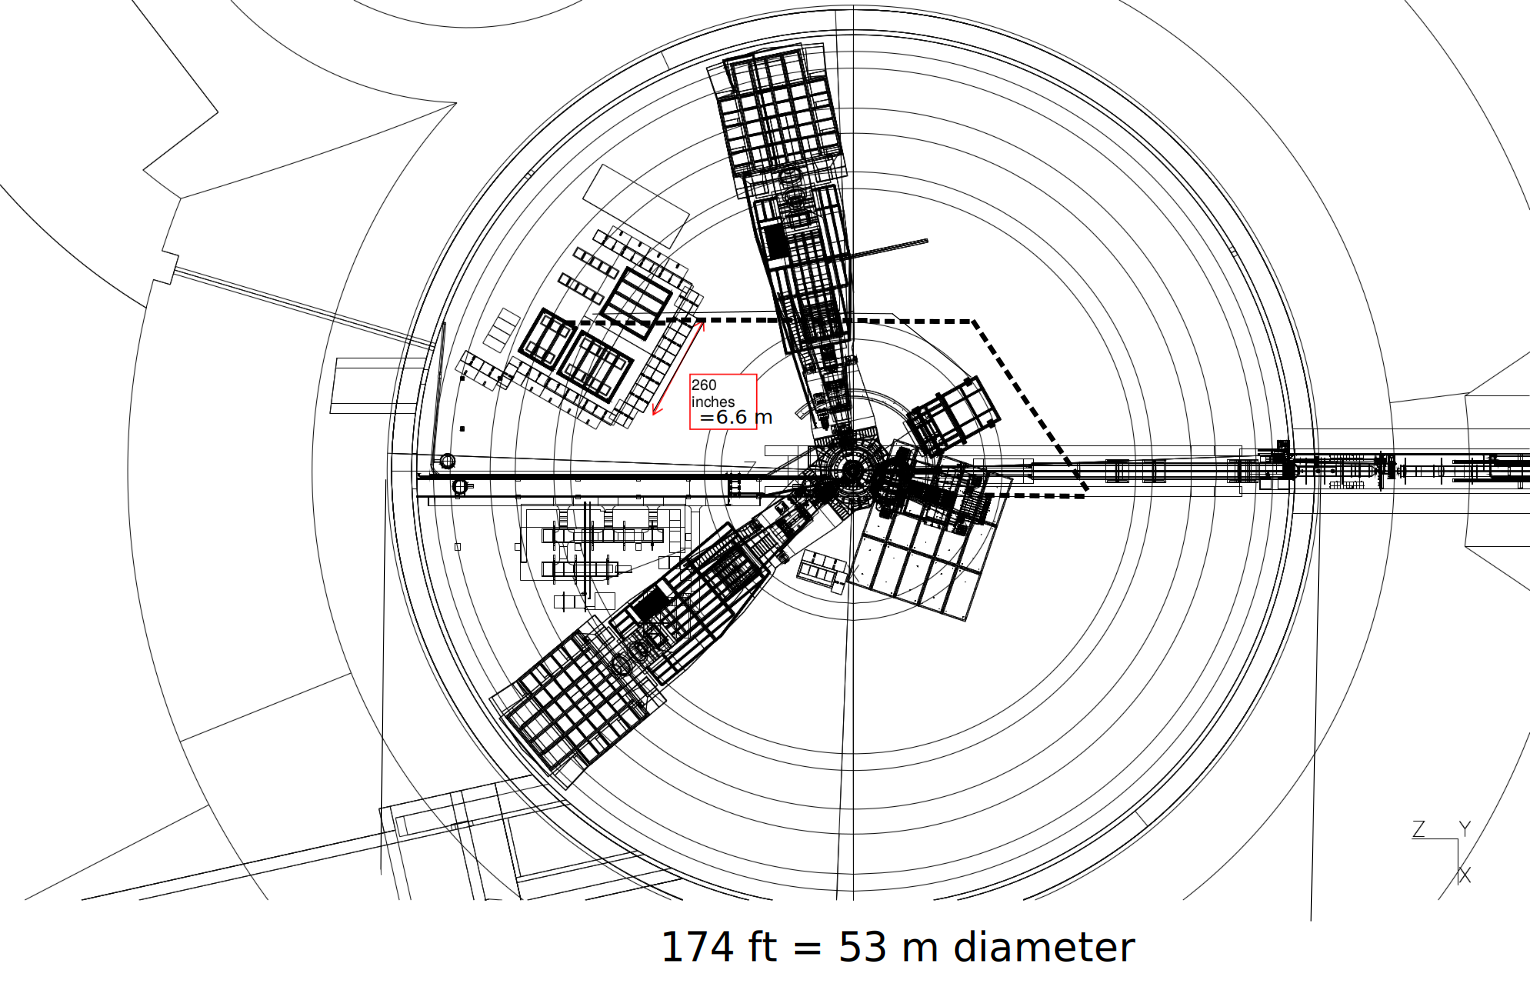
\includegraphics[scale=0.3]{figs/cablesHall.pdf}
 \section {Electronics layout}
 \includegraphics[scale=0.4]{figs/SBSlayout.pdf}

 \includegraphics[scale=0.4]{figs/FastbusEcalDetailed.pdf}

%\subsection{Fastbus}
%A special version of the trigger supervisor firmware was developped for SBS to be %able to use the event switching to different crates to reduce the dead time.
%
%
\includegraphics[scale=0.4]{figs/fastbus/TS.pdf}
%
%\includegraphics[scale=0.4]{figs/fastbus/FBCrates.pdf}
%
%Some test were carried 
%
%\includegraphics[scale=0.4]{figs/fastbus/Trigger_TS.pdf}
%
%As expected the deadtime is scaling

%\subsection{GEM readout}
% 
% 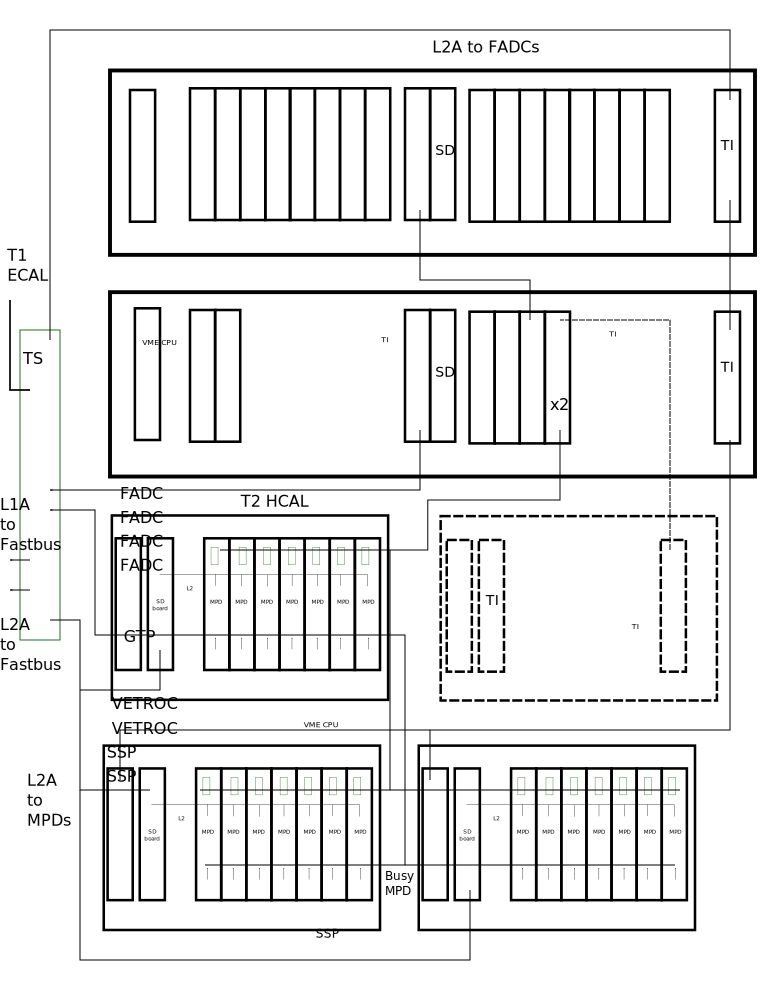
\includegraphics[scale=0.4]{figs/NewMPDDetailed.pdf}


    \end{appendices}
\end{document}
